\subsection{BỘ DỮ LIỆU}
Bộ dữ liệu sử dụng trong bài nghiên cứu lấy từ  Markets Insider (https://markets.businessinsider.com) - một trang web cung cấp tin tức thị trường chứng khoán, báo giá và biểu đồ theo thời gian thực. Bộ dữ liệu cung cấp thông tin chi tiết dữ liệu giá của 3 kim loại quý nổi bật nhất (Vàng, Bạch Kim và Palladi) trong giai đoạn từ 01/01/2018 đến 01/06/2024. Dữ liệu bao gồm các cột:\\
\indent\textbullet\ Ngày (Date): Ngày giao dịch cụ thể.\\
\indent\textbullet\ Giá mở cửa (Open): Giá của kim loại quý khi bắt đầu phiên giao dịch trong ngày.\\
\indent\textbullet\ Giá đóng cửa (Close): Giá của kim loại quý khi kết thúc phiên giao dịch trong ngày.\\
\indent\textbullet\ Giá cao nhất (High): Giá cao nhất mà kim loại quý đạt được trong phiên giao dịch.\\
\indent\textbullet\ Giá thấp nhất (Low): Giá thấp nhất mà kim loại quý đạt được trong phiên giao dịch.\\
Tuy nhiên, do mục tiêu của nghiên cứu là dự báo giá đóng cửa, nên chỉ tập trung xử lý dữ liệu liên quan đến cột "Close".Trong trường hợp có các ngày giao dịch bị thiếu dữ liệu, nội suy tuyến tính sẽ được áp dụng để ước tính giá trị đóng cửa dựa trên các giá trị liền kề đã biết, đảm bảo tính liên tục và đầy đủ của dữ liệu cho quá trình phân tích và dự báo. Công thức nội suy tuyến tính:\\
\[
 y = y1 + ((x - x1) / (x2 - x1)) * (y2 - y1)
\]
Chú thích:\\
\indent\textbullet\ y: Giá trị cần tìm.\\
\indent\textbullet\ y1: Giá trị Close của ngày gần nhất trước ngày có giá trị bị thiếu.\\
\indent\textbullet\ y2: Giá trị Close của ngày gần nhất sau ngày có giá trị bị thiếu.\\
\indent\textbullet\ x: Ngày tại giá trị cần tìm y.\\
\indent\textbullet\ x1: Ngày tại giá trị Close y1.\\
\indent\textbullet\ x2: Ngày tại giá trị Close y2.\\
\subsection{MÔ TẢ THỐNG KÊ}
\begin{table}[htbp]
  \centering
\begin{tabular}{|c|c|c|c|}
    \hline
     \  & Gold & Palladium & Platinum \\ \hline
     Count & 2344 & 2344 & 2344\\ \hline
     Mean & 1697.529 & 1719.441 & 942.257\\ \hline
     Std & 284.059 & 563.265 & 105.219\\ \hline
     Min & 1174.115 & 846 & 595\\ \hline
     25\% & 1456.6 & 1215.875 & 869.5\\ \hline
     50\% & 1778.345 & 1724.875 & 931.5\\ \hline
     75\% & 1904.25 & 2182.75 & 1000\\ \hline
     Max & 2425.49 & 3178 & 1306\\ \hline
\end{tabular}
\caption{Mô tả thống kê của vàng, paladi và bạch kim}
\end{table}

\begin{figure}[htbp]
\centerline{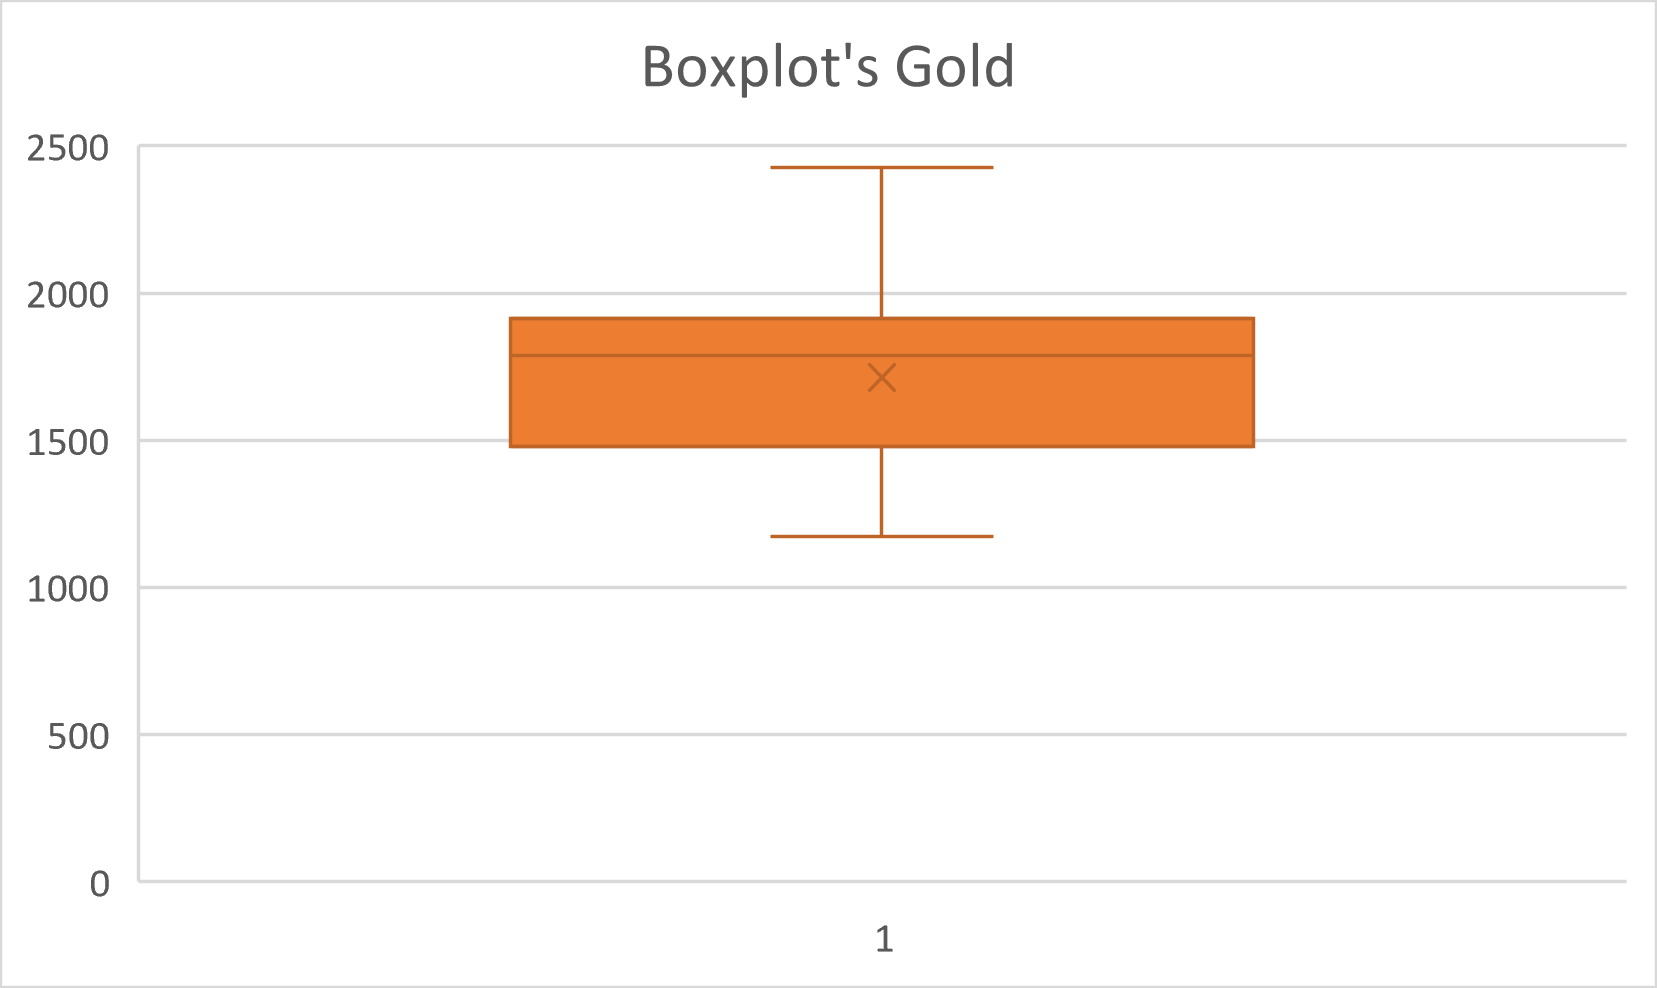
\includegraphics[width=0.4\textwidth]{img/Picture2.png}}
\caption{Sơ đồ boxplot của vàng}
\label{fig}
\end{figure}

\begin{figure}[htbp]
\centerline{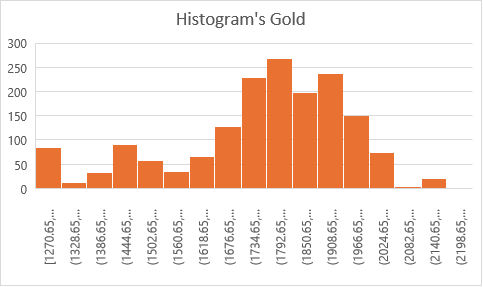
\includegraphics[width=0.4\textwidth]{img/Picture5.png}}
\caption{Sơ đồ histogram của vàng}
\label{fig}
\end{figure}

\begin{figure}[htbp]
\centerline{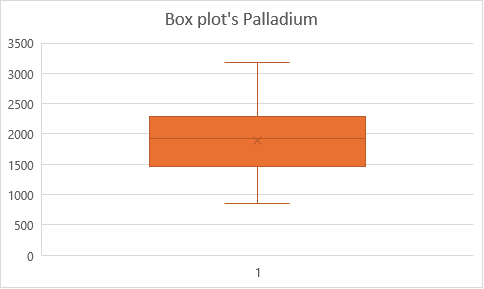
\includegraphics[width=0.4\textwidth]{img/Picture3.png}}
\caption{Sơ đồ boxplot của Paladi}
\label{fig}
\end{figure}

\begin{figure}[htbp]
\centerline{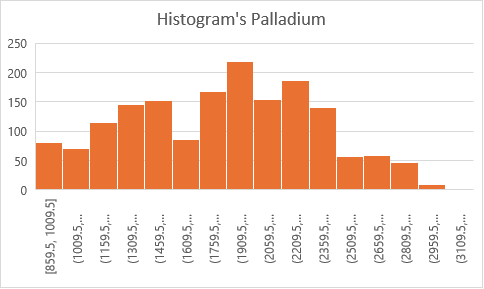
\includegraphics[width=0.4\textwidth]{img/Picture6.png}}
\caption{Sơ đồ histogram của Paladi}
\label{fig}
\end{figure}

\begin{figure}[htbp]
\centerline{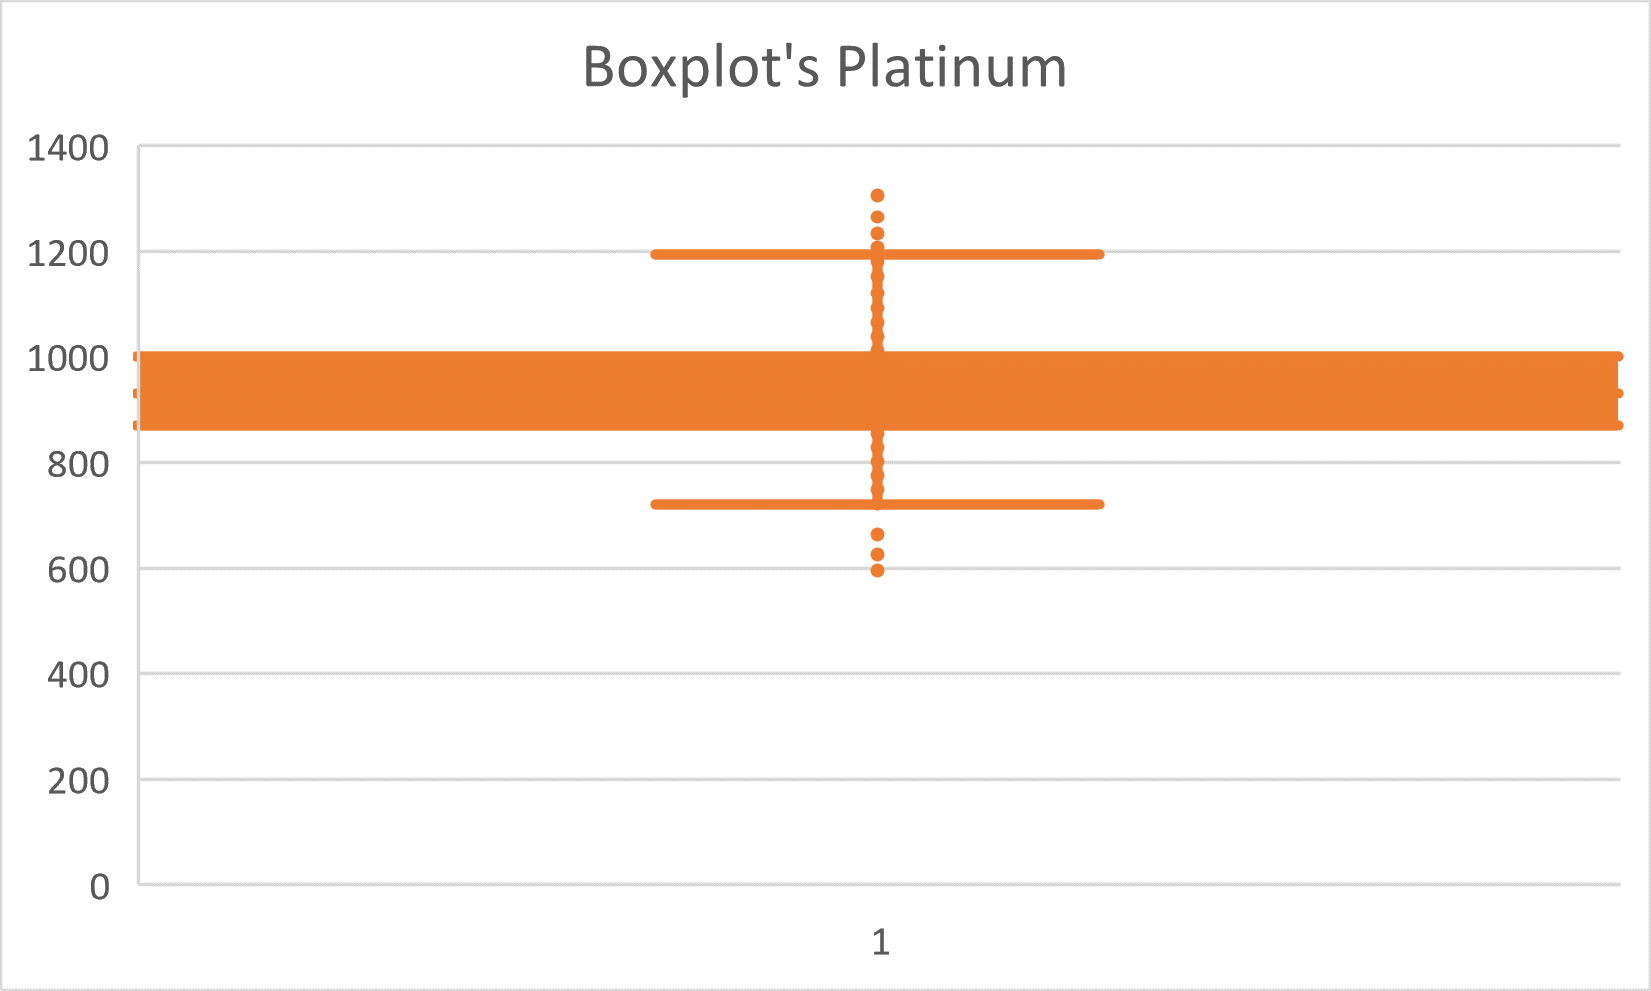
\includegraphics[width=0.4\textwidth]{img/Picture4.png}}
\caption{Sơ đồ boxplot của bạch kim}
\label{fig}
\end{figure}

\begin{figure}[htbp]
\centerline{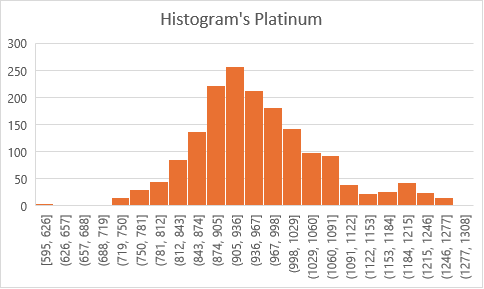
\includegraphics[width=0.4\textwidth]{img/Picture7.png}}
\caption{Sơ đồ histogram của bạch kim}
\label{fit}
\end{figure}